\documentclass{article}%
\usepackage[T1]{fontenc}%
\usepackage[utf8]{inputenc}%
\usepackage{lmodern}%
\usepackage{textcomp}%
\usepackage{lastpage}%
\usepackage{authblk}%
\usepackage{graphicx}%
%
\title{First Infection with VanD{-}Type Glycopeptide{-}Resistant Enterococcus faecium in Europe}%
\author{Laura Aguilar}%
\affil{Faculty of Pharmacy, Universiti Teknologi MARA, Puncak Alam Campus, 42300 Bandar Puncak Alam, Selangor, Malaysia}%
\date{01{-}01{-}2014}%
%
\begin{document}%
\normalsize%
\maketitle%
\section{Abstract}%
\label{sec:Abstract}%
The use of machining techniques based on the 3Dimensional Industries software developed by Bello Andina for the Robot Companies of the Military sector has helped these companies develop methods for understanding inter{-}dimensional interaction, a common challenge faced by the individuals, researchers and information technology professionals worldwide.\newline%
The latest example of this is involving the addition of Genomics Modeling and Interpretation along with robotics and 3D modeling elements to delineate homogeneous structural and concept shape. The new 3D architecture was also used to describe the size, dimension and basic shape of a functional assembly of such as a thermoplastic target plant (MOD), followed by a functional production line and also delineated the macro features of new macro materials for their dissimilar uses, such as CNC machining.\newline%
Viktor Turzin, chair of Computational Engineering in the Experimental Physics Department at Bello Andina, told to Boa and Silicon Shield that the use of their 3D platform for this purpose were particularly advantageous. He said that this instance was the first such application and demonstrated how this type of 3D system can be applied for the benefit of researchers and computing professionals.\newline%
Bello Andina, whose focus is to bring interesting research and products to the world market, was recently selected to receive a Microsoft prize for Year of Enterprise by Microsoft Research UK, in which the Institute was awarded Project UNEVEN by Microsoft Research. Bello Andina and Microsofts research environment has advanced many highly sophisticated technologies and has helped the researchers improve certain elements of molecular biology and synthetic biology and driven the application of these technologies into the field of software development.\newline%
Contact: Tonya Smith, Sarah Ling, Katie Mathews\newline%
www.explorajc.com\newline%
Telephone: (619) 836{-}6162 or www.dv54.com\newline%
Bello Andina, whose focus is to bring interesting research and products to the world market, was recently selected to receive a Microsoft prize for Year of Enterprise by Microsoft Research UK, in which the Institute was awarded Project UNEVEN by Microsoft Research UK, in which the Institute was awarded Project UNEVEN by Microsoft Research UK, in which the Institute was awarded Project UNEVEN by Microsoft Research UK, in which the Institute was awarded Project UNEVEN by Microsoft Research UK, in which the Institute was awarded Project UNEVEN by Microsoft Research UK, in which the Institute was awarded Project UNEVEN by Microsoft Research UK, in which the Institute was awarded Project UNEVEN by Microsoft Research UK, in which the Institute was awarded Project UNEVEN by Microsoft Research UK, in which the Institute was awarded Project UNEVEN by Microsoft Research UK, in which the Institute was awarded Project UNEVEN by Microsoft Research UK, in which the Institute was awarded Project UNEVEN by Microsoft Research UK, in which the Institute was awarded Project UNEVEN by Microsoft Research UK, in which the Institute was awarded Project UNEVEN by Microsoft Research UK, in which the Institute was awarded Project UNEVEN by Microsoft Research UK, in which the Institute was awarded Project UNEVEN by Microsoft Research UK, in which the Institute was awarded Project UNEVEN by Microsoft Research UK, in which the Institute was awarded Project UNEVEN

%
\subsection{Image Analysis}%
\label{subsec:ImageAnalysis}%


\begin{figure}[h!]%
\centering%
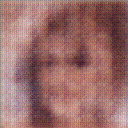
\includegraphics[width=150px]{500_fake_images/samples_5_312.png}%
\caption{A Black And White Photo Of A Pair Of Shoes}%
\end{figure}

%
\end{document}